Dans cette partie, nous présenterons un ensemble de diagrammes de séquences et de diagrammes de classes présentant le fonctionnement prévisionnel du logiciel et l’architecture qui en découle. Cette architecture tiendra compte du besoin d’extensibilité du logiciel.

\paragraph{}
Le diagramme de paquetage présenté \ref{fig:diagPaquetage} représente l’architecture globale du futur logiciel. Il montre que l'interface graphique sera le point d'entrée pour l'utilisateur. En effet,  c’est celle-ci qui redirigera les actions demandées vers soit le créateur d’image, soit le chargeur. Ce dernier sera toujours utilisé pour accéder à son attribut Scène, car il sera responsable de la création de celle-ci et de la transformation des fichiers objets en modèles 3D.

\begin{figure}[h]
		\centering
		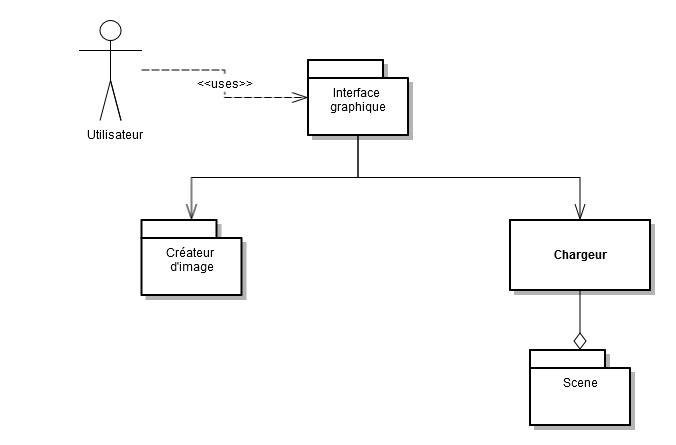
\includegraphics[scale=0.4]{diag_packages.jpg}
		\caption{\label{fig:diagPaquetage} Diagramme de paquetages}
\end{figure}

\paragraph{}
L’ensemble des diagrammes de séquence et des diagrammes de classe présentés par la suite auront été créés grâce à la version d’essai du logiciel en ligne Gliffy\footnote{\url{http://www.gliffy.com/}}.


\subsection{Diagramme de séquences}

\paragraph{}
Les diagrammes de séquence permettent de simuler les différentes communications qui auront lieu entre les classes du logiciel.

\paragraph{}
On considèrera que lorsqu’il commence à utiliser le logiciel, la première action d’un utilisateur va être de créer une scène. Grâce à l’interface graphique correspondante, qui a été présentée dans la partie Interface de ce cahier des Charges, l’utilisateur demande à l’interface de créer une scène. Celle-ci passera par l’intermédiaire d’un chargeur, déjà initialisé, qui devra créer l’instance correspondante soit à partir de rien, soit à partir d’une scène déjà existante.
    	Une fois sa tâche effectuée, le chargeur valide à l’interface qu’il a bien répondu à sa demande, et celle-ci peut modifier l’interface pour afficher la fenêtre principale, qui contient désormais la scène de travail.

\subsubsection{Création d'un objet}

\begin{figure}[h]
		\centering
		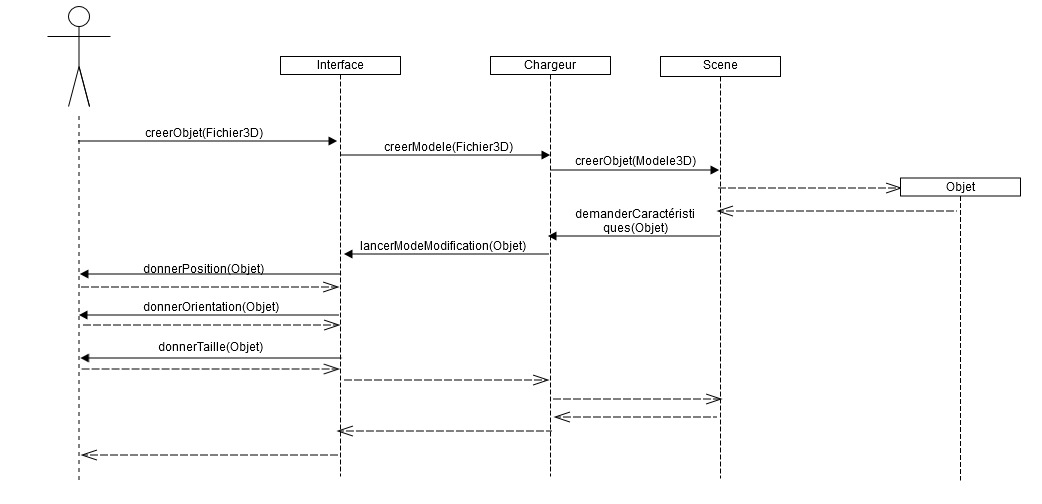
\includegraphics[scale=0.4]{creerobjet.jpg}
		\caption{\label{fig:creerObjet} Création d'un objet}
\end{figure}

\paragraph{}
Une fois la scène de travail créée, l'utilisateur pourra y ajouter des objets s'il le souhaite (cf. \ref{fig:creerObjet}). Pour cela, il va une fois de plus devoir communiquer avec l'interface graphique correspondante.

\paragraph{}
Une fois qu'il aura choisi un fichier objet d'extension .OBJ ou .PLY, l'interface enverra celui-ci au chargeur qui vérifiera sa validité et le transformera en un modèle 3D. Ce dernier sera transmis à la scène, qui se chargera de créer l'objet en plaçant les points du modèle par rapport à son origine. Ce premier objet généré sera initialisé en position centrale de la scène, avec une taille et une orientation de base définie par ses points. Enfin, une confirmation sera envoyée au chargeur, puis à l'interface, qui affichera la fenêtre correspondant au mode modification de l'objet.

\paragraph{}
Durant ce mode, l'interface demandera à l'utilisateur de modifier la position, l'orientation et la taille de l'objet s'il le souhaite, et appellera des méthodes soient publiques de l'objet, soit en passant par le chargeur puis la scène, pour effectuer les changements demandés.

\paragraph{}
Ce diagramme de séquence montre l'importance du chargeur dans l'intéraction de l'interface avec la scène. C'est lui qui s'occupera de créer la scène et de lui transmettre les demandes de l'utilisateur.


\subsubsection{Déplacement dans la scène}

\begin{figure}[h]
		\centering
		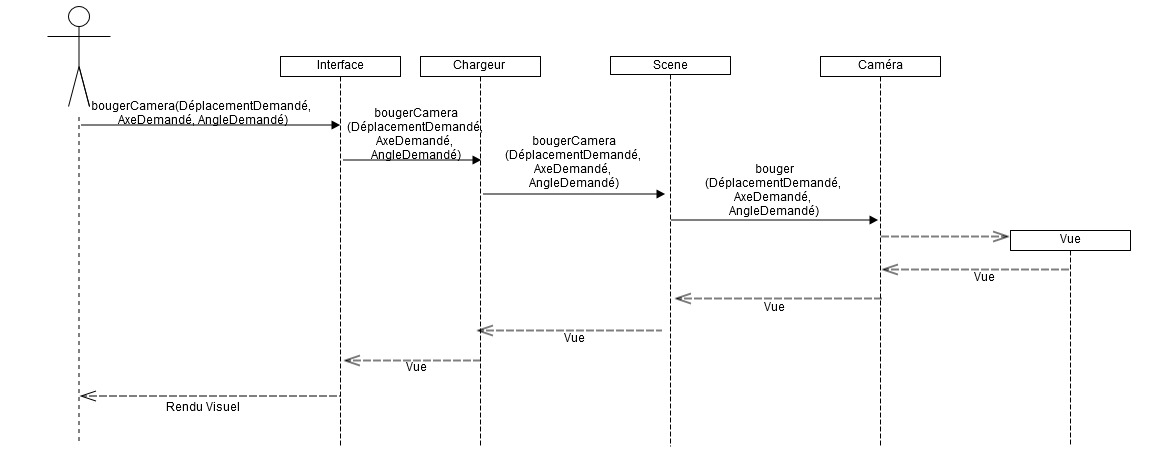
\includegraphics[scale=0.40]{bougerCamera.jpg}
		\caption{\label{fig:deplacementCam} Déplacement de la caméra}
\end{figure}

\paragraph{}
Quand il aura placé des objets dans sa scène, l’utilisateur pourra avoir envie de s’y déplacer pour observer les différents angles de vue. Pour cela, grâce à une action sur l’interface, il va demander à la caméra de se déplacer (cf. \ref{fig:deplacementCam}). La première demande sera donc initialisée par l’utilisateur, qui demandera le déplacement de la caméra à l’interface, selon un type (rotation, translation, homothétie), un axe (horizontal, vertical) et un angle ou une valeur donnée.

\paragraph{}
La caméra étant un attribut de la scène, l’interface se chargera de transmettre l’information au chargeur, qui lui-même l’enverra à la scène. Cette dernière se chargera d'appeler la fonction adéquate de son attribut qui génèrera une nouvelle vue correspondant à la projection de la scène depuis l’angle demandé par l’utilisateur. Cette vue sera renvoyée étape par étape jusqu’à l’interface, qui se chargera de la transformer en un rendu visualisable par l’utilisateur dans la zone de la scène.

\subsubsection{Création d'un autostéréogramme}

\begin{figure}[h]
		\centering
		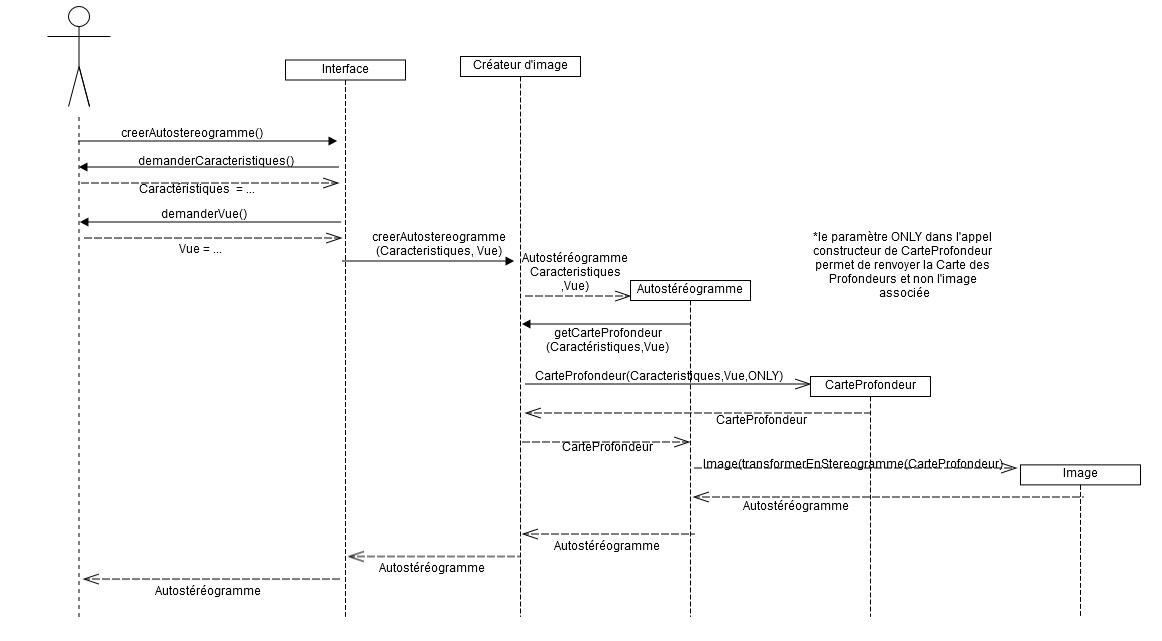
\includegraphics[scale=0.40]{creerstereogramme.jpg}
		\caption{\label{fig:creerAutostereogramme} Création d'un autostéréogramme}
\end{figure}

\paragraph{}
De la même façon que pour l’anaglyphe, c’est par l’intermédiaire de l’interface et du créateur d’image que l’utilisateur va créer son rendu (cf. \ref{fig:creerAutostereogramme}). Pour un autostéréogramme toutefois, un autre type de rendu sera également utilisé : la carte des profondeurs. C’est l’autostéréogramme qui demandera au créateur d’image de la créer pour lui, afin qu’il puisse l’utiliser pour générer l’autostéréogramme qu’il renverra vers l’utilisateur.

\newpage

\subsubsection{Création d'un flipbook}

\begin{figure}[h]
		\centering
		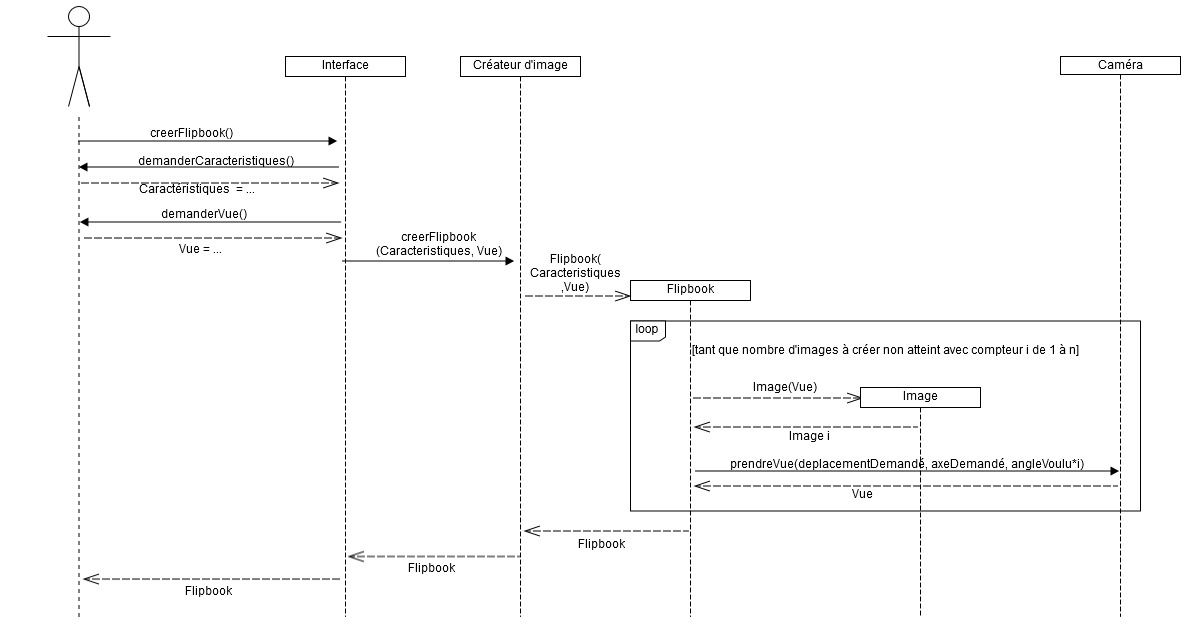
\includegraphics[scale=0.4]{creerflipbook.jpg}
		\caption{\label{fig:creerFlip} Création d'un flipbook}
\end{figure}

\paragraph{}
Une fois de plus, le passage entre l’utilisateur et le flipbook se fait par l’intermédiaire de l’interface et du créateur d’image (cf. \ref{fig:creerFlip}). Cette fois-ci toutefois, la génération se fera à l’aide d’une boucle qui permettra de remplir un vecteur d’image, qui sera renvoyé jusqu’à l’interface. Celle-ci se chargera de pouvoir afficher toutes les vues les unes après les autres dans la fenêtre d’affichage.

\paragraph{}
Les arguments deplacementDemandé, axeDemandé et angleVoulu qui sont utilisés en paramètre de la fonction prendreVue sont issus des caractéristiques choisies par l'utilisateur.

\newpage

\subsection{Diagrammes de classes}

\paragraph{}
A partir des diagrammes de séquences présentés précédemment, l’architecture du projet a pu être déterminée. La version finale de celle-ci dépendra grandement des bibliothèques OpenGL et Qt et des différentes utilisations de leurs modules.

\subsubsection{Paquetage Création}

\begin{figure}[h]
		\centering
		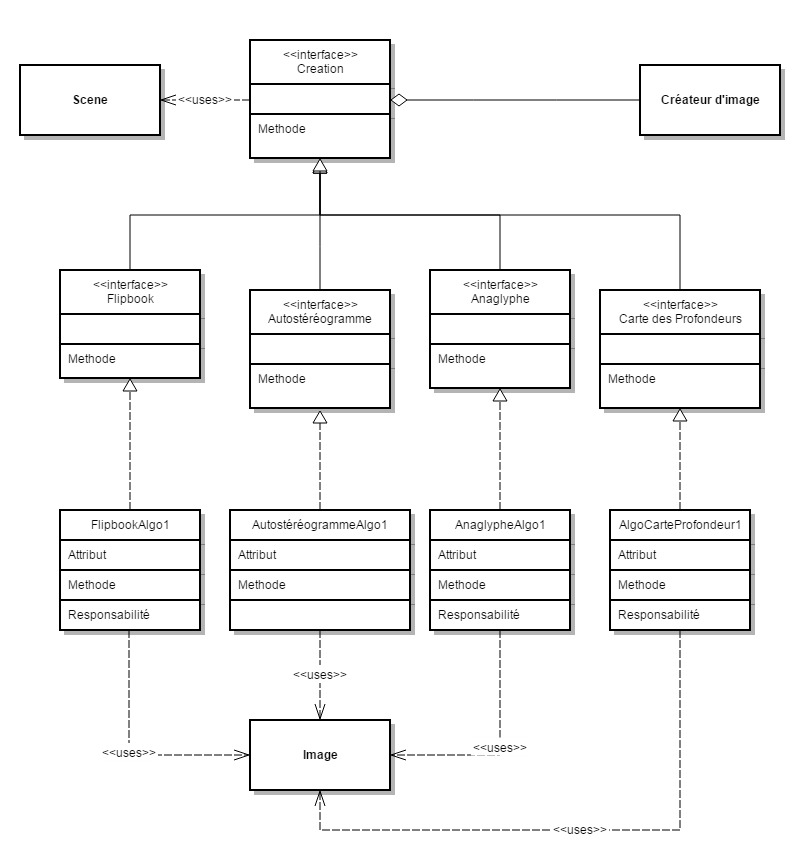
\includegraphics[scale=0.4]{package_creation.jpg}
		\caption{\label{fig:paqCreation} Architecture du paquetage Création}
\end{figure}

\paragraph{}
L’architecture du paquetage de création a été pensée pour que de futures extensions puissent être insérées à ce niveau du logiciel (cf. \ref{fig:paqCreation}). En effet, le créateur d’image génère un rendu, qui peut être l’un des types situés en dessous. Si l’on souhaite ajouter un nouveau rendu possible, il suffit donc de le placer au même niveau que les interfaces Flipbook, Autostéréogramme, etc. De la même façon, si l’on souhaite ajouter un algorithme différent pour obtenir l’un des rendus, il suffit de l’ajouter en-dessous de la classe virtuelle correspondante. Ainsi cette réalisation répond au besoin d’extensibilité.

\paragraph{}
Toutes les classes sont en relation avec la caméra par l’intermédiaire de la scène, de façon à pouvoir récupérer les différentes vues nécessaires à la création des rendus.

\newpage

\subsubsection{Paquetage Scène}

\begin{figure}[h]
		\centering
		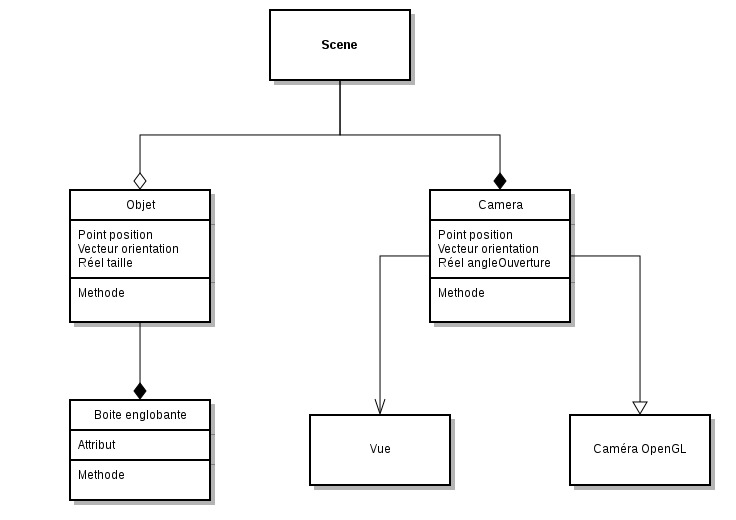
\includegraphics[scale=0.4]{paquetage_scene.jpg}
		\caption{\label{fig:paqScene} Architecture du paquetage Scène}
\end{figure}

\paragraph{}
On considèrera pour le logiciel la scène comme un ensemble d’objets et une caméra. C’est la scène qui gèrera elle-même l’accès à ses différentes composantes (cf. \ref{fig:paqScene}). La caméra utilisée, qui sera liée à la caméra de la bibliothèque OpenGL, génèrera des vues qui pourront être utilisées pour l’affichage de la scène ou la création de rendus. Le contenu réel de ces vues et leur utilisation dépendront de la bibliothèque OpenGL.

\newpage

\subsubsection{Paquetage Interface}

\begin{figure}[h]
		\centering
		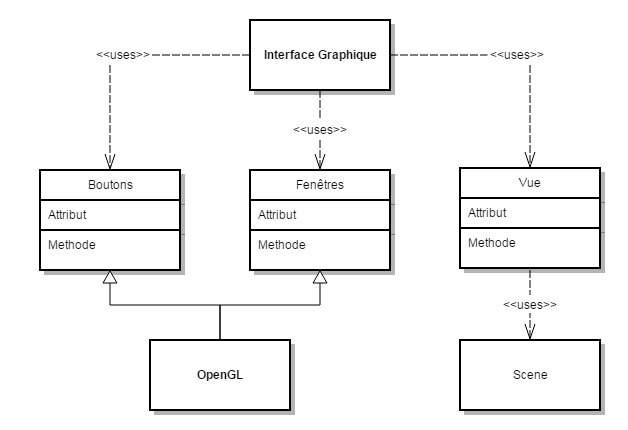
\includegraphics[scale=0.4]{package_interface.jpg}
		\caption{\label{fig:paqInterface} Architecture du paquetage Interface}
\end{figure}

\paragraph{}
Le paquetage Interface est le paquetage utilisé par l’utilisateur pour interagir avec le logiciel. L’interface sera constituée de boutons et de fenêtres, qui seront des produits de la bibliothèque Qt et du module OpenGL pour Qt (cf. \ref{fig:paqInterface}). L’affichage de la scène se fera à partir des vues générées par la Caméra de la Scène, comme expliqué dans la partie précédente.

\paragraph{}
La création de l’interface sera pensée pour que l’ajout de boutons et de fonctionnalités au logiciel se fasse de façon simple.

\newpage
